% ----- formatovani dokumentu -----------------------------------------------
\documentclass[12pt,a4paper,titlepage,final]{report}
\usepackage[utf8]{inputenc}
\usepackage[T1, IL2]{fontenc}
\usepackage{graphicx}
\usepackage{epstopdf}
\usepackage[margin=2cm]{caption}
\usepackage[top=3cm, left=2cm, right=2cm, text={17cm, 24cm}, ignorefoot]{geometry}
\usepackage{color}
\usepackage{url}
\usepackage{setspace}
\singlespacing
\usepackage[square, numbers]{natbib}
\pagestyle{plain}
\pagenumbering{arabic}
\setcounter{page}{1}
\setcounter{secnumdepth}{-1}
\setlength{\parindent}{1cm}
\usepackage{natbib}


% ----- vyberte jazyk -------------------------------------------------------
\usepackage[english,czech]{babel}
%\usepackage[english]{babel}

% ----- dopiste titulky -----------------------------------------------------
\newcommand\Course{Počítačová grafika}
\newcommand\WorkTitle{Realistické generování oblohy}
\newcommand\AuthorA{Miloslav Číž}
\newcommand\AuthorAEmail{xcizmi00@stud.fit.vutbr.cz}
\newcommand\AuthorB{Aleš Dujíček}
\newcommand\AuthorBEmail{xdujic01@stud.fit.vutbr.cz}
\newcommand\Faculty{Fakulta Informačních Technologií}
\newcommand\School{Vysoké Učení Technické v Brně}

\usepackage[
pdftitle={\WorkTitle},
pdfauthor={\AuthorA, \AuthorB},
bookmarks=true,
colorlinks=true,
breaklinks=true,
urlcolor=blue,
citecolor=blue,
linkcolor=blue,
unicode=true,
]
{hyperref}


% ----- titulni strana ------------------------------------------------------

\begin{document}
    \begin{titlepage}
    \begin{center}
        
\includegraphics[height=5cm]{images/logo.eps}
    \end{center}
    \vfill
    \begin{center}
        \begin{Large}
            \Course\\
        \end{Large}
        \bigskip
        \begin{Huge}
            \WorkTitle\\
        \end{Huge}
    \end{center}
    \vfill
    \begin{center}
        \begin{large}
            \today
        \end{large}
    \end{center}
    \vfill
    \begin{flushleft}
        \begin{large}
            \begin{tabular}{lll}
                Autoři: & \AuthorA, & \url{\AuthorAEmail} \\
                        & \AuthorB, & \url{\AuthorBEmail} \\
                & & \\
                & \Faculty \\
                & \School \\
            \end{tabular}
        \end{large}
    \end{flushleft}
\end{titlepage}

% ----- obsah --------------------------------------------------------------

\tableofcontents

% ----- zadani -------------------------------------------------------------
\newpage
\chapter{Zadání}

Zadáním bylo vytvořit program pro vhodně parametrizovatelné generování realistických obrázků oblohy za použití vhodné metody (založené např. na sledování paprsku). Měli jsme se zaměřit na vizuální kvalitu oblohy, krajinu stačilo vykreslit pouze velmi zjednodušeně. Zadání jsme upřesnili následujícím způsobem:

\begin{itemize}
    \item generování obrázků oblohy podobných fotografii
    \item metoda: sledování paprsku v kombinaci s 2D vykreslováním
    \item procedurální generování textury mraků
    \item možnost generovat sekvenci obrázků jako animaci (volitelně navazující)
\end{itemize}

%---------------------------------------------------------------------------
\chapter{Nejdůležitější dosažené výsledky}

% Popište 3 věci, které jsou na vašem projektu nejlepší. Nejlépe ukažte a
% komentujte obrázky, v nejhorším případě vypište textově.

\section{Plynulá animace}

Náš program umožňuje nad rámec zadání generovat animaci oblohy, která
může být buď mezi dvěma časovými úseky během dne, anebo během jednoho
časového okamžiku -- animace potom ve smyčce spojitě navazuje díky
spojitosti implementovaného 3D šumu.

\begin{figure}[h] \centering
        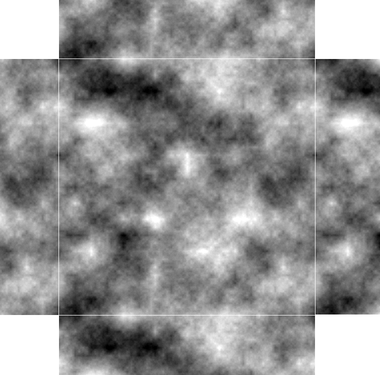
\includegraphics[width=10cm]{images/navazujici_sum.png}
    \caption{Navazující šum v prostoru} \label{fig:noise_cont_space}
\end{figure}

To, že generovaná procedurální 3D textura na sebe navazuje ve všech třech osách,
jak je vidět na obrázcích \ref{fig:noise_cont_space} a~\ref{fig:noise_cont_time},
nám umožnilo texturou posouvat a~simulovat tím pohyb mraků vlivem větru.
Návaznost textury v~čase zase způsobuje plynulou proměnlivost tvaru a~velikosti
mraků.

\begin{figure}[h] \centering
        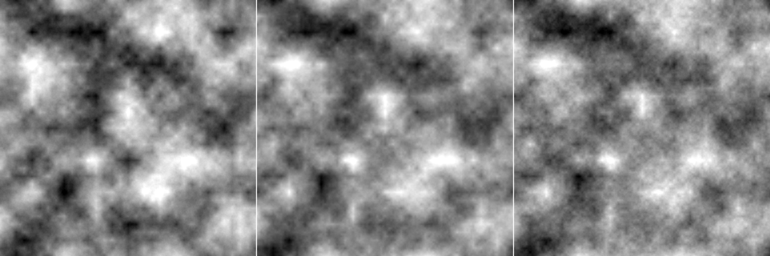
\includegraphics[width=\textwidth]{images/sum123.png}
    \caption{Navazující šum v~čase} \label{fig:noise_cont_time}
\end{figure}

\section{Zobrazení různé denní doby}

Samotná obloha je obarvena barevným přechodem, který se mení pro různou denní
dobu. Mezi těmito přechody se v~průběhu dne postupně interpoluje a~vzniká
tak efekt červánků při svítání a~západu slunce, ve dne je obloha světle modrá
a~v~noci je tma.

Toto celé ještě doplňuje Slunce a~Měsíc.

\begin{figure}[h] \centering
        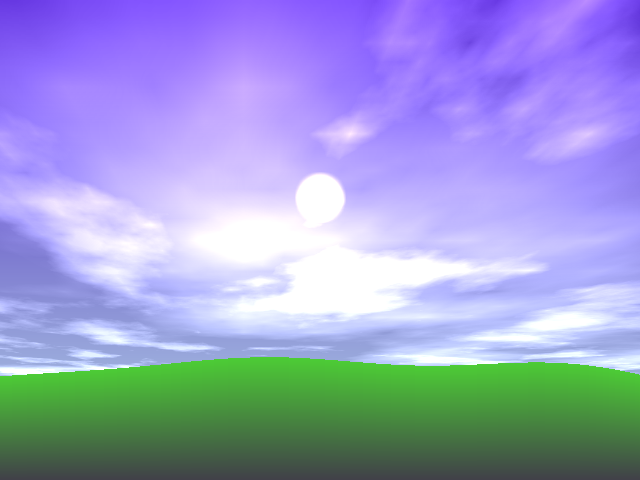
\includegraphics[width=0.5\textwidth]{images/sky0.png}
    \caption{Obloha ve dne} \label{fig:sky_day}
\end{figure}

\begin{figure}[h] \centering
        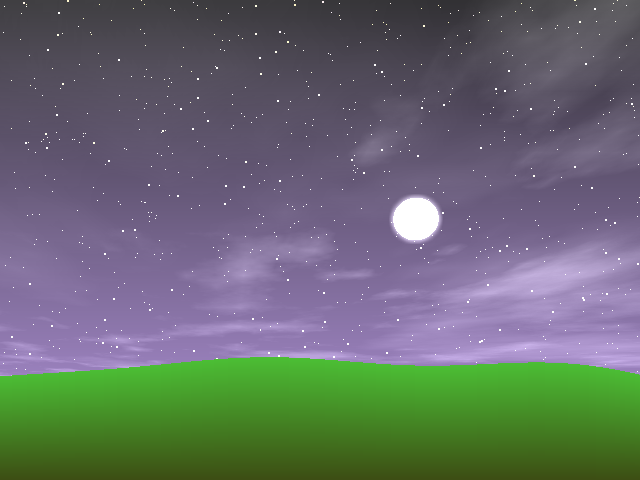
\includegraphics[width=0.5\textwidth]{images/sky1.png}
    \caption{Obloha večer} \label{fig:sky_evening}
\end{figure}

\begin{figure}[h] \centering
        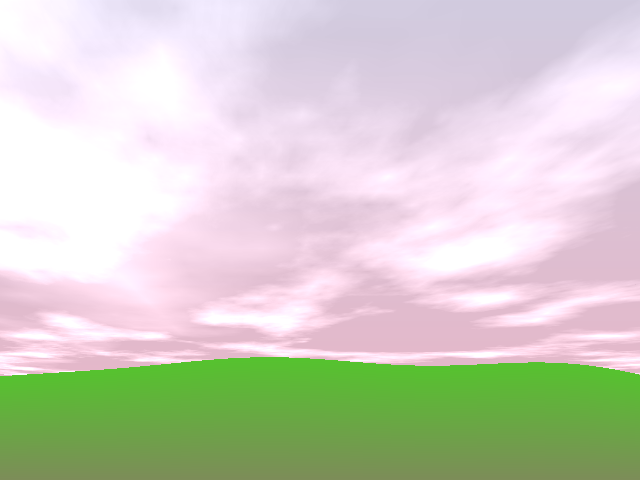
\includegraphics[width=0.5\textwidth]{images/sky2.png}
    \caption{Obloha během svítání} \label{fig:sky_dawn}
\end{figure}


\section{Paralelizace}

Z~důvodu poměrně pomalého zpracování snímku jsme se rozhodli výpočet
urychlit paralelním zpracováním. K paralelizaci jsme použili OpenMP,
které vytvoří několik vláken a~rozdělí mezi ně výpočet různých
částí snímku.

Takto se nám podařilo dosáhnout zrychlení 1,83 při zpracování dvěma
vlákny.

%---------------------------------------------------------------------------
\chapter{Zvláštní použité znalosti}

% Uveďte informace, které byly potřeba nad rámec výuky probírané na FIT.
% Vysvětlete je pomocí obrázků, schémat, vzorců apod.

Perlinův šum\cite{cite1, cite2} jsme použili k zobrazení mraků na obloze. Jde
o~šum, který vzniká jako součet několika různých náhodných signálů s~různou
frekvencí a~amlitudou.

Implementace navazující textury interpolací krajních bodů přes okraj.

% paralelizace neni pro nad ramec FIT
% \paragraph{Rozsah:} podle potřeby a vlastního uvážení

%---------------------------------------------------------------------------
\chapter{Práce na projektu}

\begin{itemize}
\item \textbf{\AuthorA}: implementace sledování paprsku, vykreslení pozadí a~krajiny, hlavní program, dokumentace
\item \textbf{\AuthorB}: implementace Perlinova šumu, animace, paralelizace, optimalizace, dokumentace
\end{itemize}

%---------------------------------------------------------------------------
\section{Co bylo nejpracnější}

% \paragraph{Rozsah:} 5-10 řádků

\begin{itemize}
\item \textbf{\AuthorA}: Sestavit scénu a~nastavit její parametry tak,
aby výstup alespoň trochu připomínal realitu. Jelikož jsem sledování
paprsku implementoval poprvé, bylo pro mě poměrně časově náročné jej
odladit.
\item \textbf{\AuthorB}: Najít vhodné parametry pro funkci, která generuje
Perlinův šum, aby výsledek nevypadal jako jediný mrak přes celou oblohu,
ale aby vznikala i místa, kterými prosvítá obloha. Problém totiž byl, že vyšší
frekvence v~Perlinově šumu byly příliš utlumeny a~neměly tak dostatečný vliv
na podobu výsledného signálu.
\end{itemize}

%---------------------------------------------------------------------------
\section{Zkušenosti získané řešením projektu}

\begin{itemize}
\item \textbf{\AuthorA}: Poprvé jsem programoval ray-tracing -- naučil
jsem se základy matematiky, která se v~této oblasti
používá (barycentrické souřadnice, výpočty průsečíků apod.). Vyzkoušel
jsem si modelování reálné přírodní scény, což jsem dosud ve škole sám
nedělal.
\item \textbf{\AuthorB}: Seznámil jsem se s~problematikou generování
procedurálních textur a~jejich mapování do scény. Vyzkoušeli jsme si
řešení konfliktů v~systému GIT. Naučil jsem se pracovat s~knihovnou SDL.
\end{itemize}

% \paragraph{Rozsah:} formulujte stručně, uchopte cca 3-5 věcí

%---------------------------------------------------------------------------
\chapter{Autoevaluace}

\paragraph{Technický návrh (85\%):}
Klíčové metody a~prostředky jsme si ujasnili před začátkem implementace
poté, co jsme projekt konzultovali. Některé věci, jako např.
supersampling, jsme přidávali až během implementace.

\paragraph{Programování (60\%):}
Kód jsme se snažili psát alespoň minimálně přehledně, objektově,
modulárně a~komentovat jej způsobem kompatibilním se systémy
pro automatické generování dokumentace. Bylo by možné
dosáhnout podstatně kvalitnějšího kódu, to však nebylo naším primárním
cílem.

\paragraph{Vzhled vytvořeného řešení (90\%):}
S~vizuálními výsledky jsme spokojeni s~ohledem na čas, který jsme na
vypracování projektu měli. Nedokonalosti v~obrázcích jsou znát např.
na mracích, pro lepší výsledky by bylo možné použít lepší druh šumu
(např. simplex noise).

\paragraph{Využití zdrojů (85\%):}
Využili jsme kód pro práci s~rastrovou grafikou a~formátem PNG napsaný v~rámci
bakalářské práce. Dále jsme využili knihovnu SDL2 a~LodePNG. Metody jsme zvolili na
základě konzultace a~studia literatury.

\paragraph{Hospodaření s časem (90\%):}
Pracovat jsme začali ihned po zadání, pokračovali jsme rovnoměrně.

\paragraph{Spolupráce v týmu (90\%):}
Snažili jsme se pracovat průběžně a~práci každý týden konzultovat. Pro
správu kódu jsme využili systém GIT.

\paragraph{Celkový dojem (90\%):}
Zadání bylo podle nás z~programátorského hlediska průměrně náročné, ale
mělo navíc umělecký aspekt, se kterým se na škole příliš nesetkáváme,
proto jsme se díky projektu hodně naučili. Výsledný program je podle
nás použitelný v~jednoduché umělecké grafice, např. pro generování pozadí
pro videa apod.

%---------------------------------------------------------------------------
\chapter{Ovládání vytvořeného programu}

\section{Technologie potřebné pro spuštění programu}
Projekt využívá tyto technologie:

\begin{itemize}
\item jazyk C++
\item překladač gcc
\item pro animaci knihovna SDL2
\end{itemize}

Program je možné přeložit a~spustit na platformách s~C++ překladačem.

\section{Obsluha programu}

Program se používá z~příkazové řádky následujícím způsobem:
{\tt skygen [[-t time][-d duration][-f frames][-o name][-c amount][-e density][-x width][-y height][-p level][-s] | [-h]]}

\begin{itemize}
\item {\tt -t} specifikuje denní dobu v~24hodinovém formátu {\tt HH:MM}.
\item {\tt -d} specifikuje trvání animace od dané denní doby celým číslem udávajícím počtet minut.
\item {\tt -f} udává počet snímků animace.
\item {\tt -o} říká, jaké bude jméno (jména) výstupního souboru.
\item {\tt -x} zadává šířku generovaného obrázku v~pixelech.
\item {\tt -y} zadává výšku generovaného obrázku v~pixelech.
\item {\tt -p} specifikuje stupeň supersamplingu.
\item {\tt -c} udává množství mraků celočíselnou hodnotou v~rozsahu 0 až 100.
\item {\tt -e} udává hustotu mraků celočíselnou hodnotou v~rozsahu 0 až 100.
\item {\tt -s} vypíná výpis zpráv během generování obrázků.
\item {\tt -h} zobrazí nápovědu.
\end{itemize}

%---------------------------------------------------------------------------
\chapter{Doporučení pro budoucí zadávání projektů}

Pozitivně hodnotíme volnost zadání projektů s~velkým prostorem pro
kreativitu a~možnost přihlásit se v~případě zájmu i~na téma, které je již
zabrané, čehož jsme sami využili.

%---------------------------------------------------------------------------

\bibliographystyle{plain}

\nocite{cite1}
\nocite{cite2}
\nocite{cite3}

\bibliography{reference}
\addcontentsline{toc}{chapter}{Literatura}

\end{document}

